% \section{Part II: Feature Extraction (for dataset B)}
% \subsection{Computing the eigenvectors and eigenvalues using PCA}
% The principle component analysis technique is used to reduce the dimensionality of the data to two dimensions. The plot in Figure~\ref{fig:fig2} shows the eigenvalues for each principle component in order of significance. Generally, a "knee" is looked for to determine how many components could be used and still retain a large amount of the variance. Overall, the components tend to decrease fairly smoothly and a knee is not overly evident. We can see a slight drop in variance from component 4 to 5. The PCA was carried out after normalizing the data using z-score.

% \begin{figure}[htb]
%  \centering
% 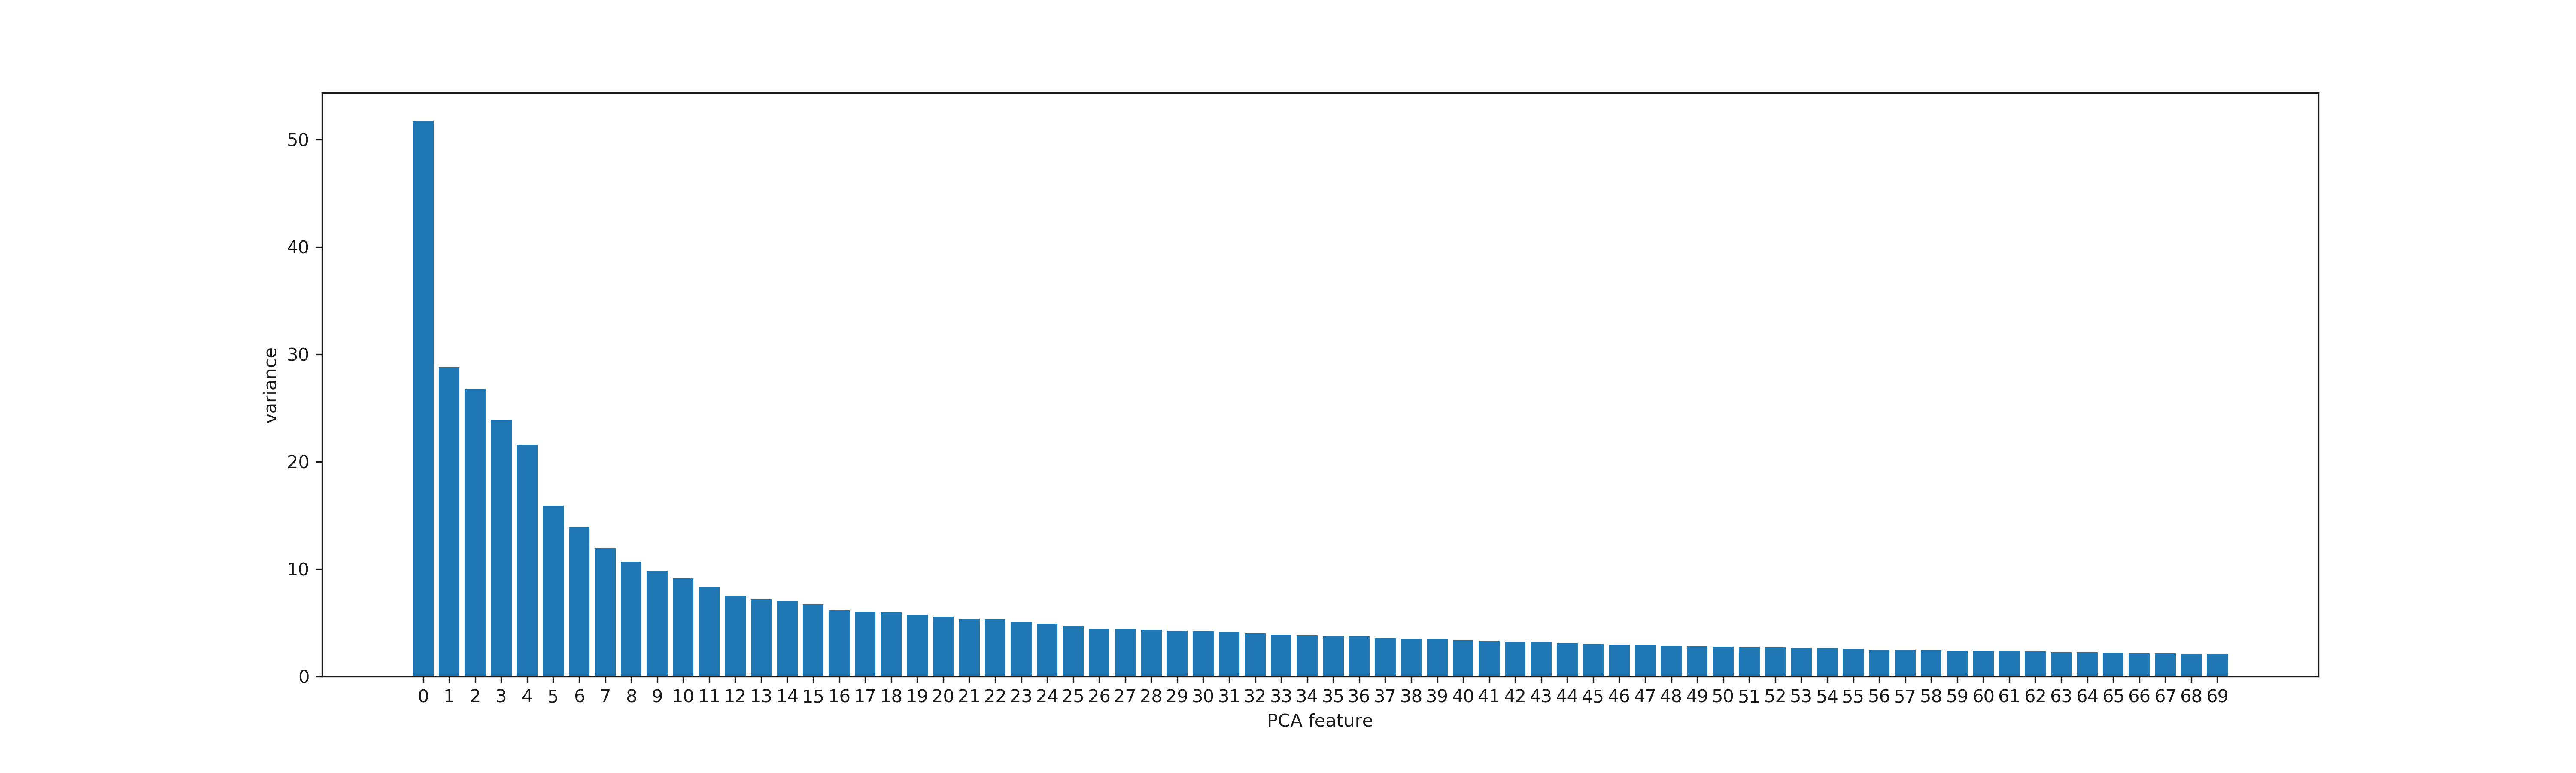
\includegraphics[width=\textwidth]{assignment1/2-1-pcafeatures.png}
% \caption{\label{fig:fig2}Scree plot showing the principal components after PCA}
% \end{figure}



% \subsection{2-D plot for the top two PCA's}

% The data is projected onto a 2 dimensional representation using the first and second principal components. The principal components are eigenvectors that represent where the data has the most variance. The projection maps the data to the plane created by the first two principal components. Figure~\ref{fig:fig3} below shows the resulting scatter plot of the data. Each digit can be identified by its colour on the plot. We can see that the digit "1" has a very tight grouping. This means that although we have attempted to maximize scatter using PCA, the features of all the hand written "1's" in the dataset are still very similar. We can contrast this by observing the digit "0". This digit has the largest spread compared to any other number. This indicates that the values of features vary greatly between different hand written "0's" and as a result could be harder to group and classify.

% \begin{figure}[htb]
%  \centering
% 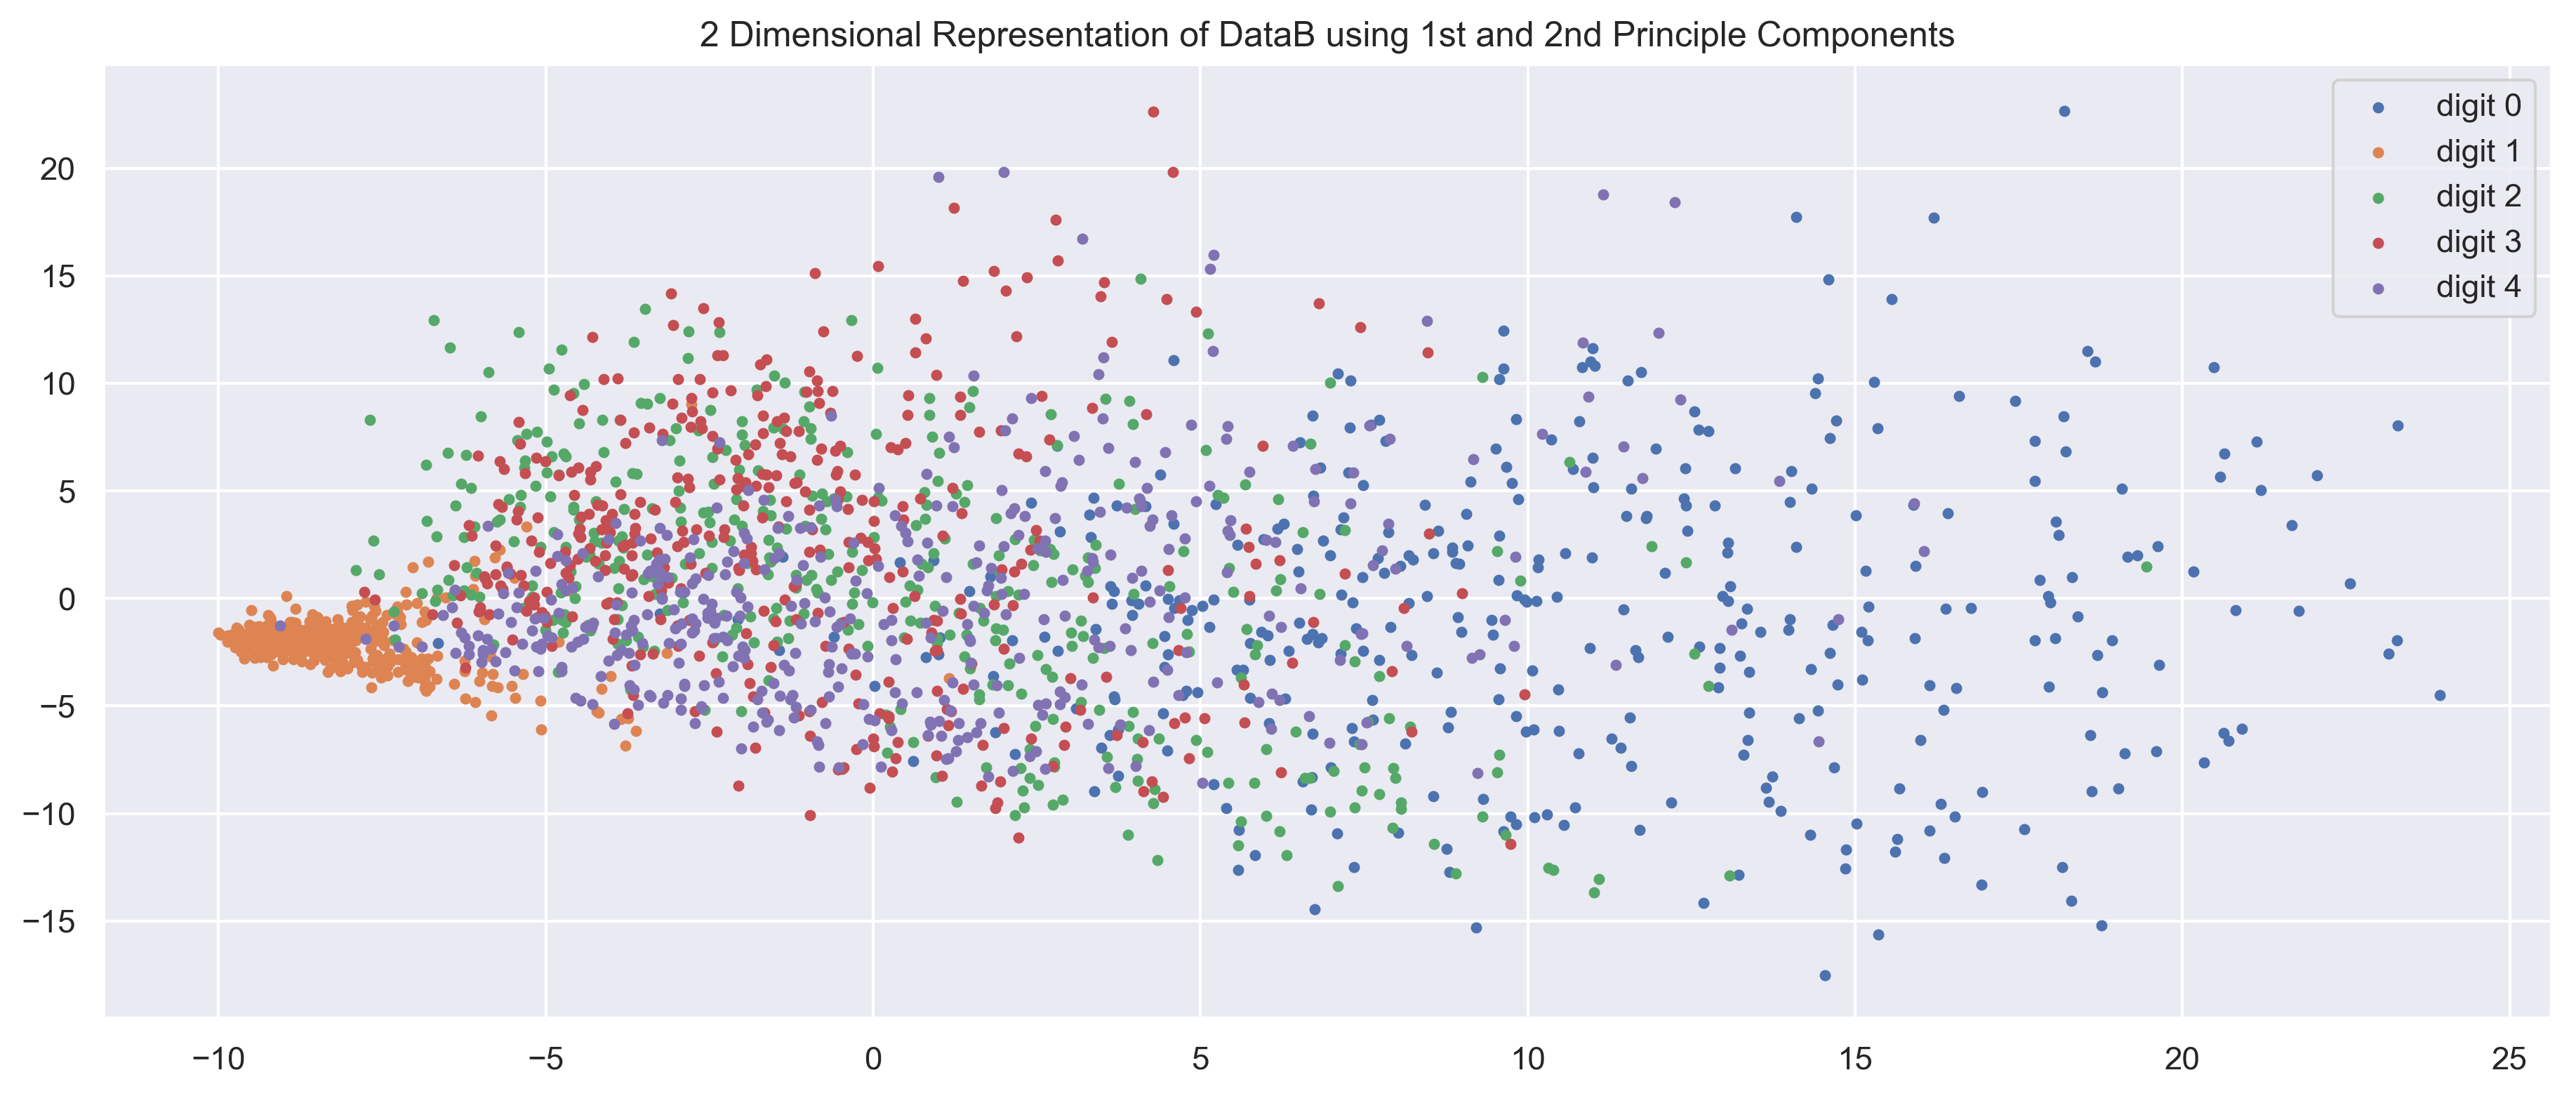
\includegraphics[width=\textwidth]{assignment1/2-2-dimreduction_pca1_2.png}
% \caption{\label{fig:fig3}Data reduced to 2 dimensions using the first and second principal components}
% \end{figure}


% \clearpage{}
% \subsection{2-D plot for the 5th and 6th principal components}

% The PCA projection was repeated using the 5th and 6th principal components. We would expect that these principal components contain less variance than the PCA features used in Figure~\ref{fig:fig3}. A similar plot was created by mapping the data to the plane created by the 5th and 6th components. This was done manually in our code because the PCA class offered by sci-kit learn does not have an option to select a range of PCA components starting from an arbitrary component. The eigenvectors were retrieved from the model and the transpose was right multiplied by the data. The result is similar to above, and can be seen in Figure~\ref{fig:fig4}. As we expected, the variance contained in these components is lower and as a result the data points are grouped together more. It is harder to distinguish the digits from one another as they all tend to have a similar amount of scatter and appear centered around the mean. We can also see that the maximum spread of the data is much less than in Figure~\ref{fig:fig3}. Qualitatively, PCA using the first two components spreads from -10 to 20 while the 5th and 6th components result in a spread of -10 to 10.

% \begin{figure}[htb]
%  \centering
% 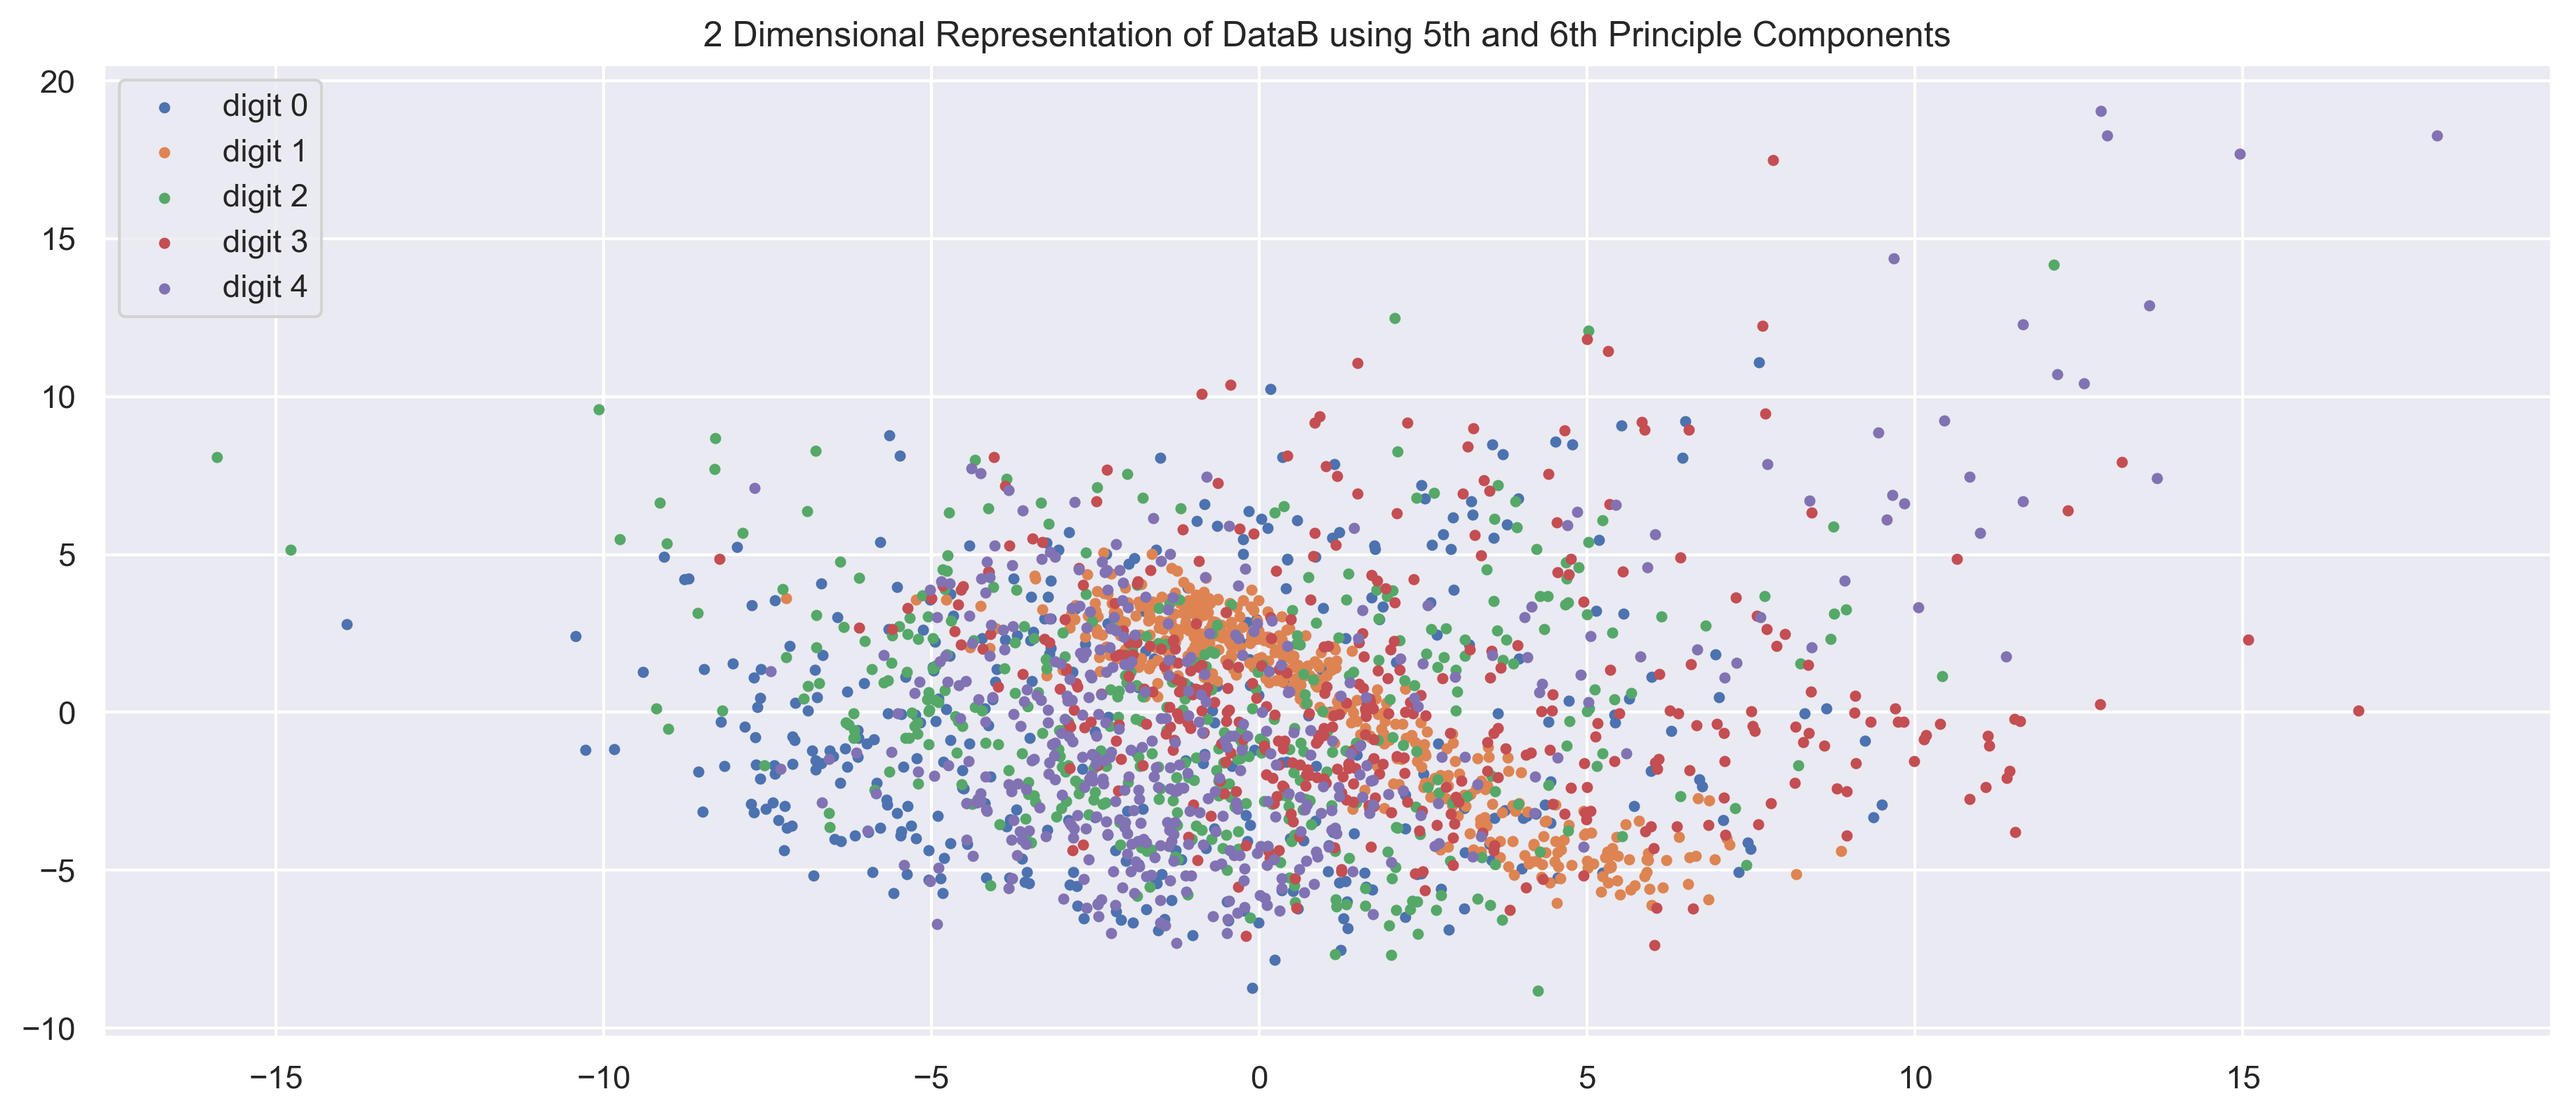
\includegraphics[width=\textwidth]{assignment1/2-3-dimreduction_pca5_6.png}
% \caption{\label{fig:fig4}Data reduced to 2 dimensions using the fifth and sixth principal components}
% \end{figure}



% \clearpage{}
% \subsection{Naive Bayes classifier for 8 sets of dimensionality reduced data}

% The dataset was transformed in 8 sets of differing dimensionality. A Naive Bayes model was applied to each set and trained using the labels provided. Accuracy of the model was determined by directly predicting the label given the data it was trained on. Naive Bayes is a simple linear hypothesis function and as a result, it is highly susceptible to bias, however, it is resilient to over-fitting.  Figure~\ref{fig:fig5} shows a bar plot of each set and its corresponding performance.  Figure~\ref{fig:fig6} show a line plot of performance vs the variance retained in the set after the dimensionality reduction. It is interesting to see that performance improves with more retained variance up to a point. The performance of the Naive Bayes classifier is best when the dimensionality reduction retains approximately 43\% of the variance. After that point performance declines. One hypothesis for this result is that as we provide more information by including additional features (dimensions), the classifier has to model much more variance. This noise could cause problems in predictive power because the it dilutes the information with the most influential predictive power (the first few principal components). Perhaps applying a technique to split the data into training and testing data could improve results.  
% \begin{figure}[htb]
%  \centering
% 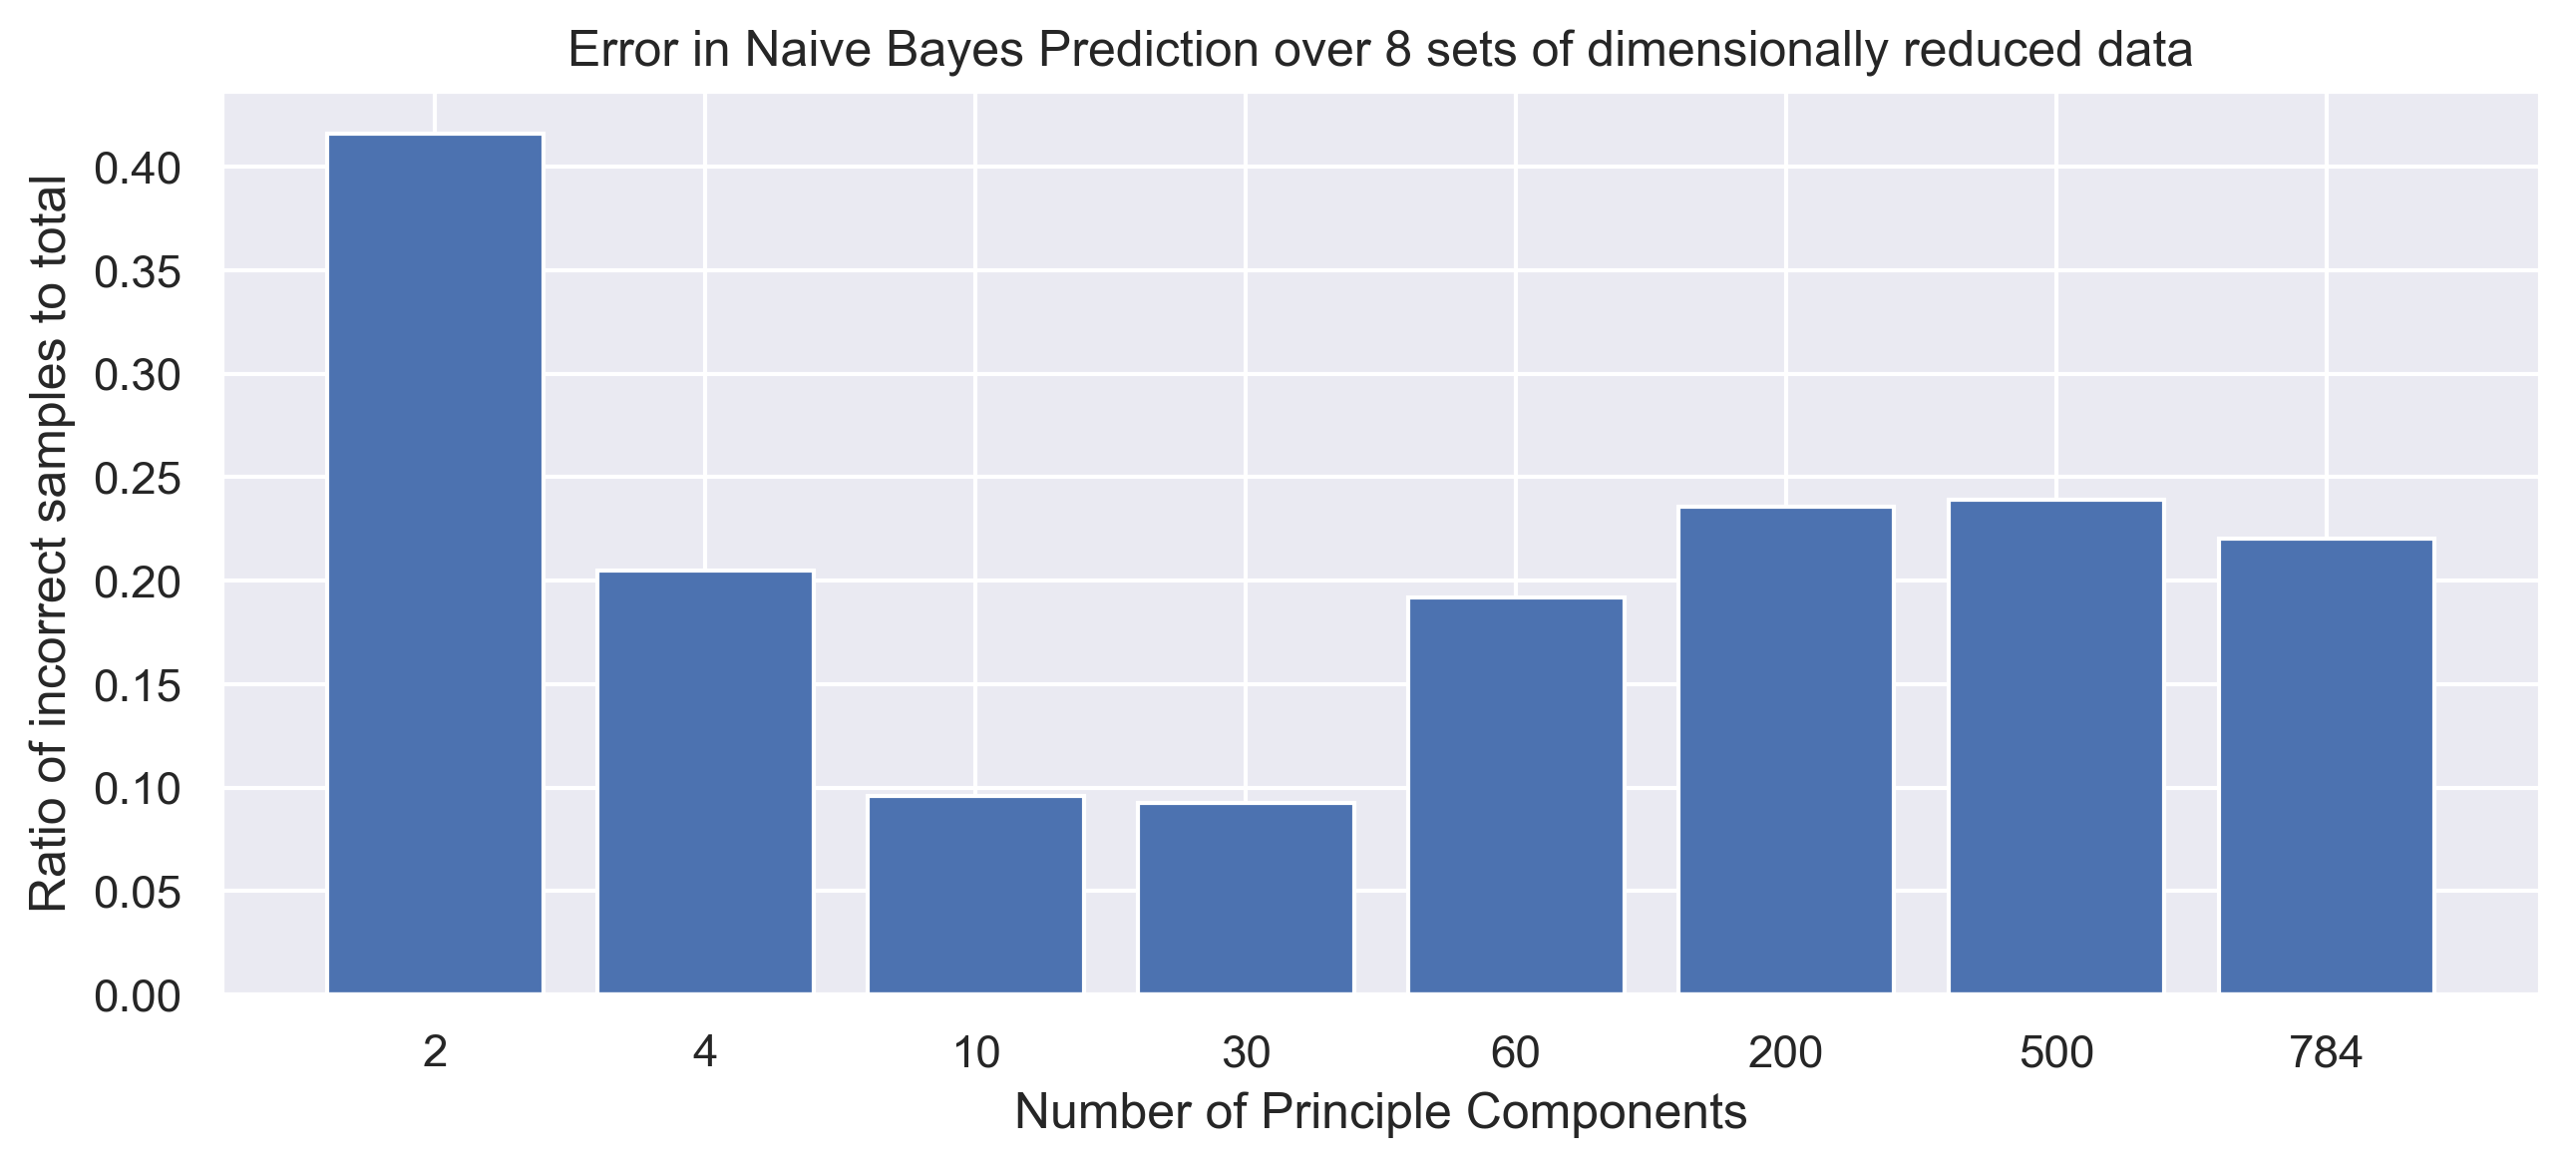
\includegraphics[width=\textwidth]{assignment1/2-4-NBprediction_bar.png}
% \caption{\label{fig:fig5}Naive Bayes classifier performance over multiple sets of dimensionality reduced data}
% \end{figure}

% \begin{figure}[htb]
%  \centering
% 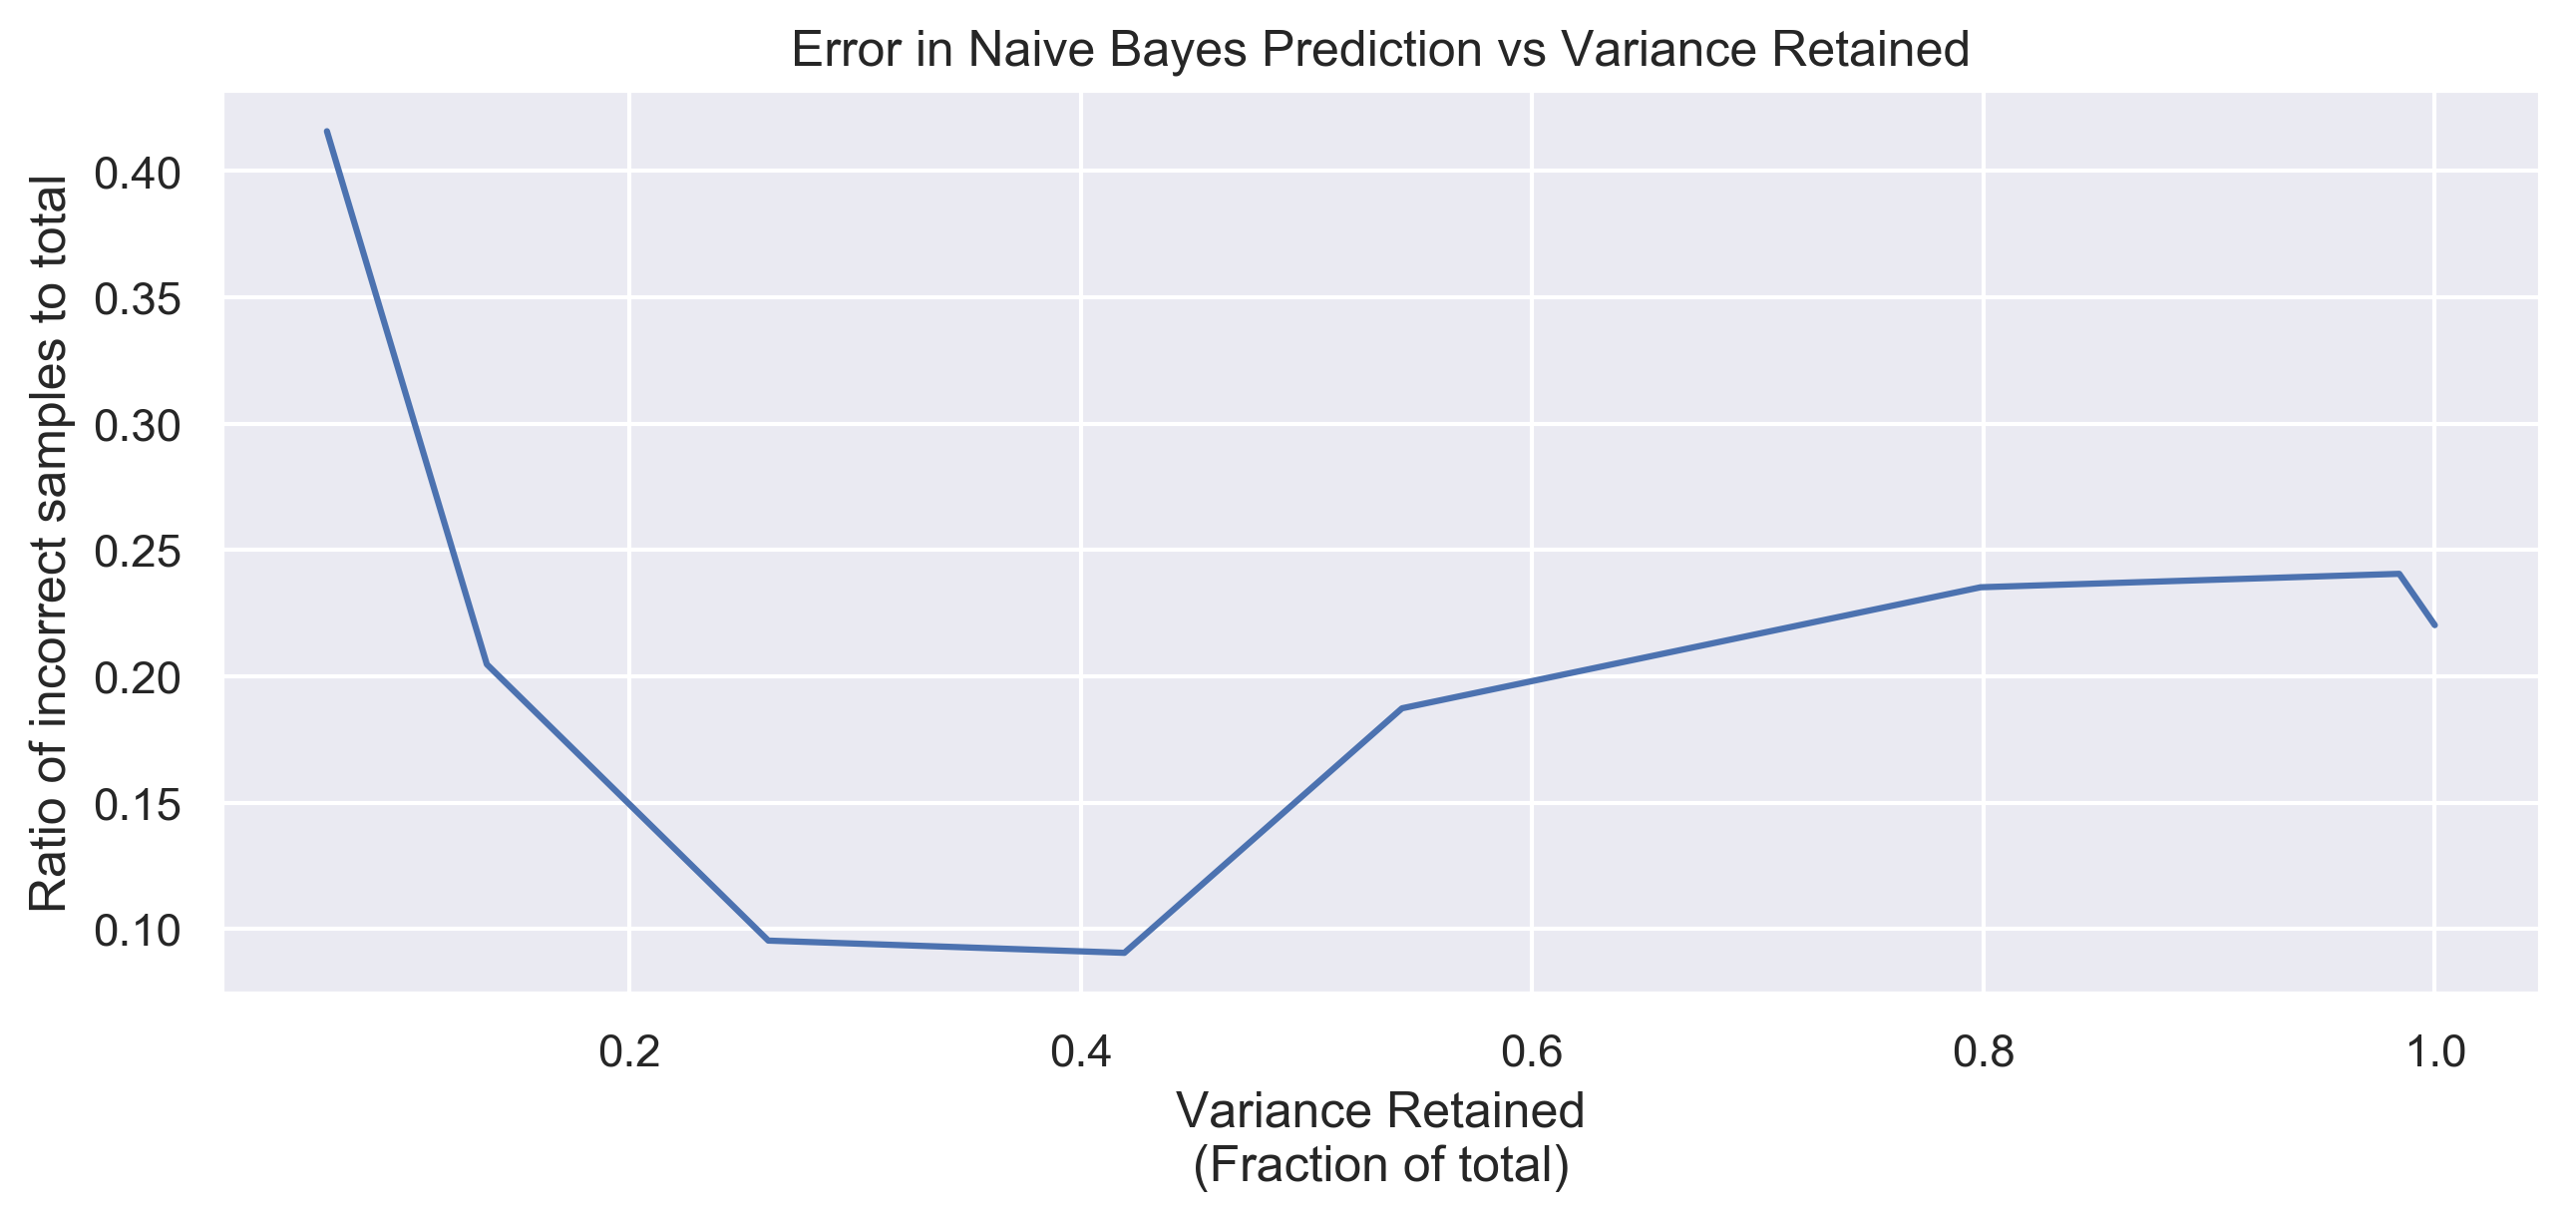
\includegraphics[width=\textwidth]{assignment1/2-4-NBprediction_line.png}
% \caption{\label{fig:fig6}Naive Bayes classifier performance versus the variance retained in the training set}
% \end{figure}


% \clearpage{}
% \subsection{Linear Discriminant Analysis (LDA)}

% Linear discriminant analysis was used to reduce the dimensionality of the data to 2 dimensions. Figure~\ref{fig:fig7} shows a scatter plot of the data after the LDA transformation. Each class is coloured in different colour. The LDA technique seems to group the classes very well. It is easy to distinguish the boundaries between the different digits of the data. The PCA transformation result in groupings where it is not intuitive to discern the class. This is most likely due to the fact that the two techniques differ in their approach. LDA is a supervised technique that uses the class labels to determine boundaries between the labels. Since PCA is unsupervised, it does not have the ability to map each class relative to one another and simply aims to maximize scatter and variance between the features.

% \begin{figure}[htb]
%  \centering
% 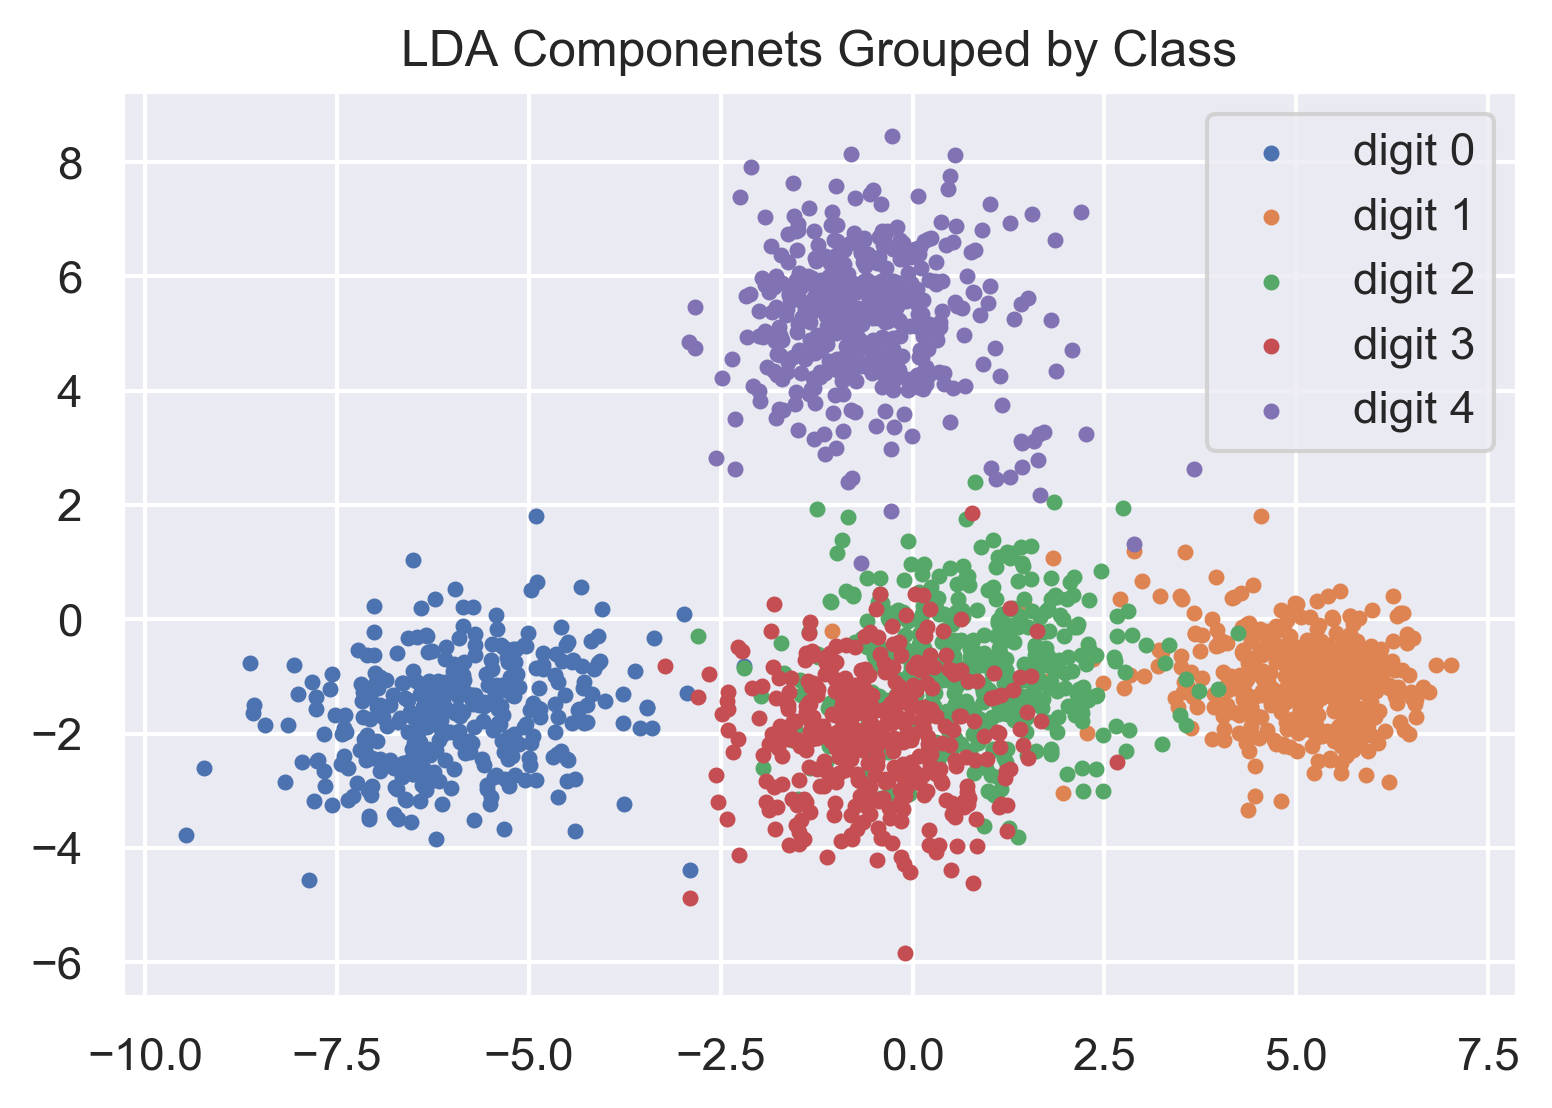
\includegraphics[width=\textwidth]{assignment1/2-5-LDA_dim_reduction.png}
% \caption{\label{fig:fig7}LDA dimension reduction to 2 dimensions}
% \end{figure}